\documentclass[13pt,a4paper]{article}
\usepackage[utf8]{inputenc}
\usepackage[T1]{fontenc}
\usepackage{lmodern}
\usepackage{geometry}
\geometry{margin=2cm}
\usepackage{graphicx}
\usepackage{hyperref}
\usepackage{listings}
\usepackage{xcolor}
\usepackage{float}
\usepackage{booktabs}
\usepackage{titling}
\usepackage{fancyhdr}
\usepackage{tcolorbox}
\usepackage{setspace}
\usepackage{titlesec}

% Enhanced typography
\onehalfspacing

% Define code listing style
\definecolor{codegreen}{rgb}{0,0.6,0}
\definecolor{codegray}{rgb}{0.5,0.5,0.5}
\definecolor{codepurple}{rgb}{0.58,0,0.82}
\definecolor{backcolour}{rgb}{0.95,0.95,0.95}

\lstdefinestyle{mystyle}{
    backgroundcolor=\color{backcolour},   
    commentstyle=\color{codegreen},
    keywordstyle=\color{blue},
    stringstyle=\color{codepurple},
    basicstyle=\ttfamily\small,
    breakatwhitespace=false,         
    breaklines=true,                 
    captionpos=b,                    
    keepspaces=true,                  
    showspaces=false,                
    showstringspaces=false,
    showtabs=false,                  
    tabsize=2,
    frame=single,
}

\lstset{style=mystyle}

% Hyperref setup
\hypersetup{
    colorlinks=true,
    linkcolor=blue,
    filecolor=magenta,
    urlcolor=blue,
    pdftitle={Court Kart: E-Commerce Database Implementation},
    pdfauthor={HADJ ARAB Adel},
    pdfsubject={E-Commerce Database},
    pdfkeywords={e-commerce, database, triggers, stored procedures, MySQL}
}

% Page style setup
\pagestyle{fancy}
\fancyhf{}
\fancyhead[R]{\thepage}
\fancyhead[L]{Court Kart E-Commerce}
\renewcommand{\headrulewidth}{0.4pt}

% Title formatting
\pretitle{\begin{center}\LARGE\bfseries}
\posttitle{\end{center}\vskip 0.5em}
\preauthor{\begin{center}\large}
\postauthor{\end{center}}
\predate{\begin{center}\large}
\postdate{\end{center}}

\renewcommand{\contentsname}{\centerline{TABLE OF CONTENTS}}

\begin{document}

% Custom title page
\begin{titlepage}
	\centering
	\vspace*{1cm}

	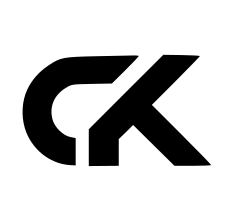
\includegraphics[width=0.4\textwidth]{../public/assets/images/court-kart-logo.png}\\[1.5cm]

	\textbf{\LARGE Court Kart: E-Commerce Platform}\\[0.5cm]
	\textbf{\Large Database Implementation Project}\\[2cm]

	\begin{minipage}{0.45\textwidth}
		\begin{flushleft}
			\large
			\textbf{Submitted by:}\\
			HADJ ARAB Adel\\
			Student ID: 222231482117\\
		\end{flushleft}
	\end{minipage}

	\vfill

	{\large \today}

\end{titlepage}

% Table of contents on separate page
\newpage
\tableofcontents
\newpage

\section{Introduction}

Court Kart is a specialized e-commerce platform designed for basketball enthusiasts. The platform offers a wide range of basketball-related products including footwear, apparel, gear, and merchandise. This report documents the database implementation of the platform, focusing on its relational schema, stored procedures, triggers, and the overall integration with the web application.

The database design follows best practices for e-commerce applications, with particular attention to inventory management, order processing, and user account management. The implementation leverages MySQL's advanced features such as stored procedures and triggers to ensure data integrity, automate processes, and enhance application performance.

\section{Database Design}

\subsection{Relational Schema and Relationships}

Court Kart's database is structured around the following core entities and relationships:

\begin{itemize}
	\item \textbf{users}: Stores user account information including authentication details, profile data, and role assignment (user/admin)
	\item \textbf{products}: Contains comprehensive product details including inventory levels, pricing information, categorization, and media assets
	\item \textbf{cart\_items}: Represents the shopping cart functionality, linking users to products they intend to purchase
	\item \textbf{orders}: Records order transactions with status tracking and financial details
	\item \textbf{order\_items}: Contains the line items within each order, maintaining historical pricing data
	\item \textbf{canceled\_orders}: Records history and reasons for canceled transactions
	\item \textbf{logs}: Maintains a comprehensive audit trail of system operations
\end{itemize}

\subsubsection{Key Relationships}

\begin{itemize}
	\item One user can have many cart items (one-to-many)
	\item One user can place many orders (one-to-many)
	\item One order contains many order items (one-to-many)
	\item Each product can appear in many carts and orders (many-to-many through junction tables)
	\item One canceled order references exactly one order (one-to-one)
	\item System logs can reference users and orders (many-to-one)
\end{itemize}

\begin{figure}[H]
	\centering
	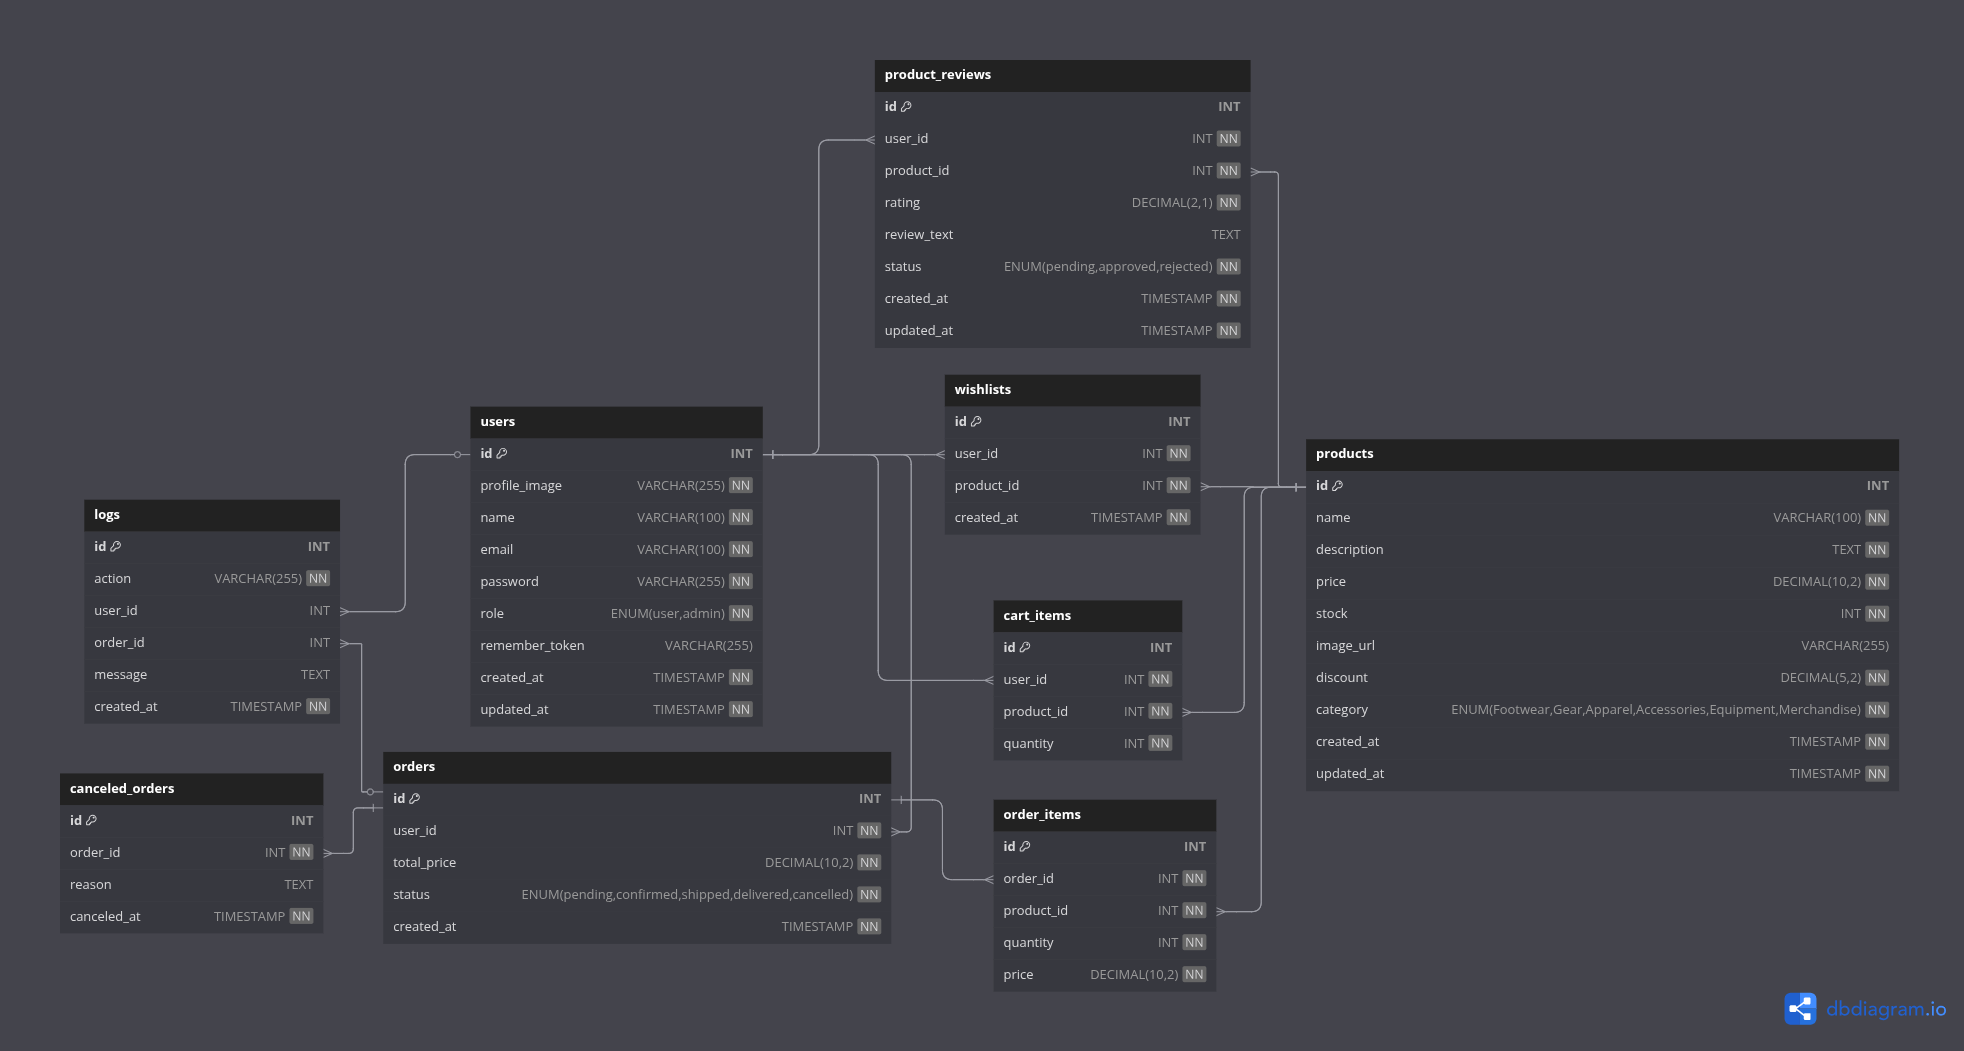
\includegraphics[width=0.9\textwidth]{../public/assets/images/db-schema.png}
	\caption{Entity-Relationship Diagram for Court Kart Database}
\end{figure}

\subsection{Schema Optimization and Constraints}

The database schema incorporates several optimization strategies:

\begin{itemize}
	\item \textbf{Appropriate data types}: Selected to minimize storage requirements while ensuring data integrity
	\item \textbf{Foreign key constraints}: Implemented to maintain referential integrity across related tables
	\item \textbf{CHECK constraints}: Applied to validate data (e.g., ensuring discount values are between 0 and 1)
	\item \textbf{ENUM types}: Used for fields with predefined values to enforce data consistency
	\item \textbf{Indexing}: Applied to frequently queried columns to improve performance
	\item \textbf{Default values}: Provided where appropriate to simplify data insertion
\end{itemize}

\section{Stored Procedures Implementation}

Stored procedures are utilized to encapsulate complex business logic and improve application performance. The following key procedures have been implemented:

\subsection{GetOrderDetails Procedure}
This procedure retrieves comprehensive details about a specific order, joining multiple tables to provide a complete view of the transaction.

\begin{lstlisting}[language=SQL]
CREATE PROCEDURE GetOrderDetails (IN p_order_id INT)
BEGIN
    SELECT
        o.id AS order_id,
        o.created_at AS order_date,
        o.status,
        u.name AS customer_name,
        u.email AS customer_email,
        p.id AS product_id,
        p.name AS product_name,
        p.image_url,
        oi.quantity,
        oi.price AS unit_price,
        (oi.quantity * oi.price) AS subtotal,
        o.total_price AS total_amount
    FROM
        orders o
        JOIN users u ON o.user_id = u.id
        JOIN order_items oi ON o.id = oi.order_id
        JOIN products p ON oi.product_id = p.id
    WHERE
        o.id = p_order_id;
END
\end{lstlisting}

\subsubsection{Implementation Notes}
This procedure:
\begin{itemize}
	\item Joins four tables to compile complete order information
	\item Calculates subtotals for each line item
	\item Returns both individual product details and aggregate order information
	\item Supports administrative and customer-facing order viewing
\end{itemize}

\subsection{FinalizeOrder Procedure}
This procedure handles the critical order checkout process, ensuring data consistency through transaction management.

\begin{lstlisting}[language=SQL]
CREATE PROCEDURE FinalizeOrder (
    IN p_order_id INT,
    IN p_user_id INT
)
BEGIN
    DECLARE v_order_exists INT;

    START TRANSACTION;

    SELECT COUNT(*) INTO v_order_exists
    FROM orders
    WHERE id = p_order_id AND user_id = p_user_id AND status = 'pending';

    IF v_order_exists = 1 THEN
        UPDATE orders
        SET status = 'confirmed'
        WHERE id = p_order_id;

        DELETE FROM cart_items
        WHERE user_id = p_user_id;

        INSERT INTO logs (action, user_id, order_id, message)
        VALUES ('CHECKOUT', p_user_id, p_order_id, 'Order finalized and cart emptied');

        COMMIT;
    ELSE
        ROLLBACK;
        SIGNAL SQLSTATE '45000'
        SET MESSAGE_TEXT = 'Invalid or non-pending order for this user';
    END IF;
END
\end{lstlisting}

\subsubsection{Implementation Notes}
This procedure:
\begin{itemize}
	\item Validates order existence and ownership before processing
	\item Uses transactions to ensure atomicity of multi-step operations
	\item Clears the user's cart after successful order confirmation
	\item Logs the checkout action for audit purposes
	\item Provides error handling with descriptive messages
\end{itemize}

\subsection{GetCustomerOrderHistory Procedure}
This procedure retrieves a customer's complete order history with aggregated product information.

\begin{lstlisting}[language=SQL]
CREATE PROCEDURE GetCustomerOrderHistory (
    IN p_user_id INT
)
BEGIN
    SELECT
        o.id AS order_id,
        o.created_at AS order_date,
        o.total_price,
        o.status,
        COUNT(oi.id) AS item_count,
        GROUP_CONCAT(p.name SEPARATOR ', ') AS products
    FROM
        orders o
        LEFT JOIN order_items oi ON o.id = oi.order_id
        LEFT JOIN products p ON oi.product_id = p.id
    WHERE
        o.user_id = p_user_id
    GROUP BY
        o.id, o.created_at, o.total_price, o.status
    ORDER BY
        o.created_at DESC;
END
\end{lstlisting}

\subsubsection{Implementation Notes}
This procedure:
\begin{itemize}
	\item Uses LEFT JOINs to include all orders, even if they have no items
	\item Employs GROUP\_CONCAT to create a comma-separated list of product names
	\item Counts items per order for quick reference
	\item Orders results chronologically for intuitive display
\end{itemize}

\section{Triggers Implementation}

Triggers automate critical business logic and maintain data integrity across the database. The following key triggers have been implemented:

\subsection{AfterOrderConfirmed Trigger}
This trigger automatically updates product stock quantities when an order status changes to 'confirmed'.

\begin{lstlisting}[language=SQL]
CREATE TRIGGER AfterOrderConfirmed
AFTER UPDATE ON orders
FOR EACH ROW
BEGIN
    DECLARE v_done INT DEFAULT 0;
    DECLARE v_product_id INT;
    DECLARE v_quantity INT;
    DECLARE cur CURSOR FOR 
        SELECT product_id, quantity FROM order_items WHERE order_id = NEW.id;
    DECLARE CONTINUE HANDLER FOR NOT FOUND SET v_done = 1;

    IF OLD.status != 'confirmed' AND NEW.status = 'confirmed' THEN
        INSERT INTO logs (action, user_id, order_id, message)
        VALUES ('CHECKOUT', NEW.user_id, NEW.id, CONCAT('Order #', NEW.id, ' confirmed'));

        OPEN cur;
        read_loop: LOOP
            FETCH cur INTO v_product_id, v_quantity;
            IF v_done THEN
                LEAVE read_loop;
            END IF;
            UPDATE products
            SET stock = stock - v_quantity
            WHERE id = v_product_id;
        END LOOP;
        CLOSE cur;
        
        INSERT INTO logs (action, user_id, order_id, message)
        VALUES ('PRODUCT_UPDATE', NEW.user_id, NEW.id, CONCAT('Stock updated for order #', NEW.id));
    END IF;
END
\end{lstlisting}

\subsubsection{Implementation Notes}
This trigger:
\begin{itemize}
	\item Uses a cursor to iterate through all order items
	\item Only activates when an order status specifically changes to 'confirmed'
	\item Automatically decrements product stock levels
	\item Creates log entries before and after stock updates for audit purposes
\end{itemize}

\subsection{BeforeOrderItemInsert Trigger}
This trigger prevents adding items to orders if the requested quantity exceeds available stock.

\begin{lstlisting}[language=SQL]
CREATE TRIGGER BeforeOrderItemInsert
BEFORE INSERT ON order_items
FOR EACH ROW
BEGIN
    DECLARE available_stock INT;
    DECLARE v_user_id INT;
    
    SELECT stock INTO available_stock
    FROM products
    WHERE id = NEW.product_id;
    
    SELECT user_id INTO v_user_id
    FROM orders
    WHERE id = NEW.order_id;

    IF NEW.quantity > available_stock THEN
        INSERT INTO logs (action, user_id, order_id, message)
        VALUES ('PRODUCT_UPDATE', v_user_id, NEW.order_id, 
                CONCAT('Failed to add product #', NEW.product_id, ' to order #', NEW.order_id, 
                       ': Requested ', NEW.quantity, ', Available ', available_stock));
                
        SIGNAL SQLSTATE '45000'
        SET MESSAGE_TEXT = 'Cannot insert order item: requested quantity exceeds available stock';
    END IF;
END
\end{lstlisting}

\subsubsection{Implementation Notes}
This trigger:
\begin{itemize}
	\item Acts as a gatekeeper before inserting order items
	\item Compares requested quantity against available stock
	\item Creates detailed log entries when stock limitations are encountered
	\item Throws a descriptive error message when insertion fails
\end{itemize}

\subsection{AfterOrderCancelled and LogCanceledOrder Triggers}
These complementary triggers restore product stock when orders are canceled and maintain a history of canceled orders.

\begin{lstlisting}[language=SQL]
-- Only showing part of these triggers for brevity
CREATE TRIGGER AfterOrderCancelled
AFTER UPDATE ON orders
FOR EACH ROW
BEGIN
    -- ... existing code ...
    
    IF OLD.status != 'cancelled' AND NEW.status = 'cancelled' THEN
        -- Log the order cancellation
        INSERT INTO logs (action, user_id, order_id, message)
        VALUES ('ORDER_CANCEL', NEW.user_id, NEW.id, CONCAT('Order #', NEW.id, ' canceled'));
        
        -- Restore product stock using cursor
        -- ... existing code ...
    END IF;
END
\end{lstlisting}

\subsubsection{Implementation Notes}
These triggers:
\begin{itemize}
	\item Work together to handle order cancellation workflows
	\item Restore product stock quantities automatically
	\item Create audit trail entries
	\item Maintain historical records of cancellations for reporting
\end{itemize}

\section{Product Data Structure and Management}

The Court Kart database maintains a comprehensive product catalog with carefully structured data:

\subsection{Product Categories}
Products are organized into six primary categories:
\begin{itemize}
	\item \textbf{Footwear}: Basketball shoes from major brands (Nike, Adidas, Under Armour)
	\item \textbf{Apparel}: Jerseys, shorts, and other clothing items
	\item \textbf{Gear}: Support equipment like ankle braces and protective gear
	\item \textbf{Accessories}: Complementary items like headbands, water bottles, and bags
	\item \textbf{Equipment}: Core basketball equipment like balls, pumps, and training aids
	\item \textbf{Merchandise}: Collectibles, posters, and fan items
\end{itemize}

\subsection{Inventory Management}
The platform implements robust inventory management through:
\begin{itemize}
	\item Real-time stock tracking via database triggers
	\item Automatic stock deduction upon order confirmation
	\item Stock restoration when orders are canceled
	\item Prevention of orders that exceed available stock
	\item Comprehensive logging of inventory transactions
\end{itemize}

\section{Logging and Auditing}

The Court Kart database implements comprehensive logging capabilities:

\subsection{Log Types}
The system tracks various event types:
\begin{itemize}
	\item User authentication events (USER\_REGISTER, USER\_LOGIN, USER\_LOGOUT)
	\item Cart operations (CART\_ADD, CART\_REMOVE)
	\item Order processing (CHECKOUT, ORDER\_UPDATE, ORDER\_CANCEL)
	\item Inventory management (PRODUCT\_ADD, PRODUCT\_UPDATE, PRODUCT\_DELETE)
\end{itemize}

\subsection{Log Structure and Implementation}
Each log entry contains:
\begin{itemize}
	\item Action type (using ENUM for consistency)
	\item User ID (when applicable)
	\item Order ID (when applicable)
	\item Detailed message explaining the event
	\item Timestamp for chronological tracking
\end{itemize}

The logs table is indexed on action type and timestamp to support efficient querying for administrative reporting and troubleshooting.

\section{Website Implementation Overview}

The Court Kart web application layers on top of the database infrastructure to provide a complete e-commerce experience:

\subsection{Key Features}
\begin{itemize}
	\item \textbf{Product browsing and search}: Allows customers to navigate the catalog with filtering options
	\item \textbf{User account management}: Supports registration, authentication, and profile management
	\item \textbf{Shopping cart system}: Provides temporary storage of selected items before checkout
	\item \textbf{Order management}: Facilitates the complete order lifecycle including tracking and history
	\item \textbf{Admin dashboard}: Offers inventory management, order processing, and reporting for administrators
\end{itemize}

\subsection{Security Measures}
The application implements several security measures:
\begin{itemize}
	\item Parameterized queries to prevent SQL injection
	\item Password hashing for secure credential storage
	\item Input validation at application and database levels
	\item Role-based access control for administrative functions
	\item Comprehensive logging for audit and security monitoring
\end{itemize}

\section{Conclusion}

The Court Kart database implementation demonstrates best practices for e-commerce data management with special attention to:

\begin{itemize}
	\item Data integrity through constraints, triggers, and stored procedures
	\item Performance optimization through appropriate indexing and query design
	\item Business logic encapsulation in database operations
	\item Security and auditing through comprehensive logging
	\item Scalable design to support future growth
\end{itemize}

The combination of a well-structured relational database with automated processes creates a robust foundation for the Court Kart e-commerce platform, enabling efficient operations and a seamless customer experience.

\end{document}
